% Self-play training loop diagram
% Compile with: pdflatex system_selfplay.tex
\documentclass[tikz,border=2pt]{standalone}
\usepackage{amsmath}
\usetikzlibrary{arrows.meta,positioning,shapes.geometric,fit,backgrounds,calc}

\begin{document}
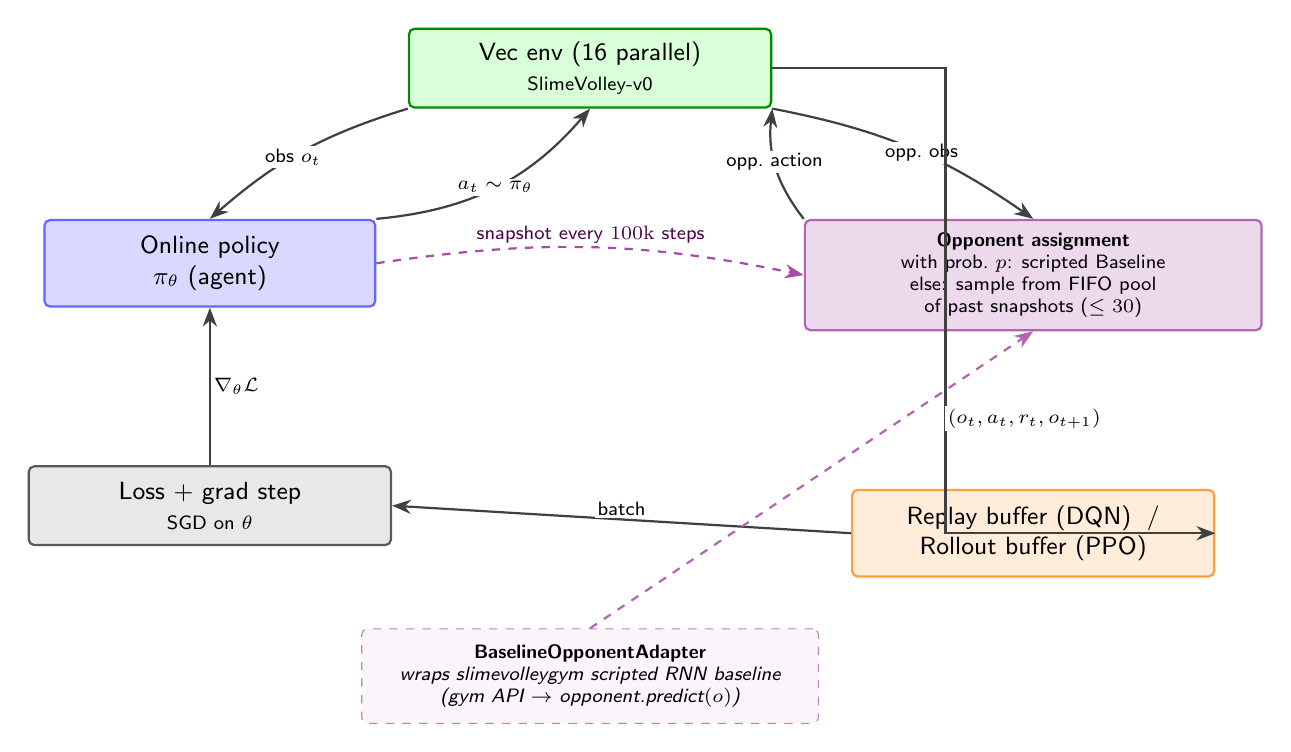
\begin{tikzpicture}[
  font=\sffamily\small,
  >={Stealth[length=2.4mm,width=1.8mm]},
  envbox/.style={
    draw, rounded corners=2pt, thick,
    minimum width=46mm, minimum height=10mm,
    align=center, fill=green!15, draw=green!55!black
  },
  agentbox/.style={
    draw, rounded corners=2pt, thick,
    minimum width=42mm, minimum height=11mm,
    align=center, fill=blue!15, draw=blue!60
  },
  oppbox/.style={
    draw, rounded corners=2pt, thick,
    minimum width=58mm, minimum height=14mm,
    align=center, fill=violet!15, draw=violet!60,
    font=\sffamily\scriptsize
  },
  bufbox/.style={
    draw, rounded corners=2pt, thick,
    minimum width=46mm, minimum height=11mm,
    align=center, fill=orange!15, draw=orange!75
  },
  lossbox/.style={
    draw, rounded corners=2pt, thick,
    minimum width=46mm, minimum height=10mm,
    align=center, fill=gray!18, draw=black!65
  },
  inset/.style={
    draw, rounded corners=2pt, thin, dashed,
    minimum width=58mm, minimum height=12mm,
    align=center, fill=violet!4, draw=violet!50,
    font=\sffamily\scriptsize\itshape
  },
  arr/.style={->, thick, draw=black!75},
  rolllbl/.style={font=\sffamily\scriptsize, fill=white, inner sep=1pt},
  notelbl/.style={font=\sffamily\scriptsize\itshape, text=black!55}
]

% =============================================================
% top: vec env
% =============================================================
\node[envbox] (env) {Vec env (16 parallel)\\\scriptsize SlimeVolley-v0};

% center row: agent <-- opponent assignment --> opponent pool
\node[agentbox, below left=14mm and 4mm of env] (agent)
   {Online policy\\$\pi_{\theta}$ (agent)};

\node[oppbox, below right=14mm and 4mm of env] (opp)
   {\textbf{Opponent assignment}\\
    with prob.\ $p$: scripted Baseline\\
    else: sample from FIFO pool\\
    of past snapshots ($\le 30$)};

% bottom row: replay/rollout buffer + loss
\node[bufbox, below=20mm of opp] (buf)
   {Replay buffer (DQN) \;/\\Rollout buffer (PPO)};

\node[lossbox, below=20mm of agent] (loss)
   {Loss + grad step\\\scriptsize SGD on $\theta$};

% inset: BaselineOpponentAdapter
\node[inset, below=20mm of env, yshift=-46mm] (adapter)
   {\textbf{BaselineOpponentAdapter}\\
    wraps slimevolleygym scripted RNN baseline\\
    (gym API $\to$ opponent.predict$(o)$)};

% =============================================================
% arrows
% =============================================================

% env -> agent (observations)
\draw[arr] (env.south west) to[bend right=12]
   node[rolllbl, pos=0.55] {obs $o_t$} (agent.north);

% env -> opponent assignment (observations for opponent)
\draw[arr] (env.south east) to[bend left=12]
   node[rolllbl, pos=0.55] {opp.\ obs} (opp.north);

% agent -> env (action)
\draw[arr] (agent.north east) to[bend right=22]
   node[rolllbl, pos=0.5] {$a_t \sim \pi_{\theta}$} (env.south);

% opponent -> env (opp action)
\draw[arr] (opp.north west) to[bend left=22]
   node[rolllbl, pos=0.55] {opp.\ action} (env.south east);

% env -> buffer (transitions)
\draw[arr] (env.east) -| ++(22mm,-30mm) |-
   node[rolllbl, pos=0.25, xshift=10mm]
        {$(o_t, a_t, r_t, o_{t+1})$} (buf.east);

% buffer -> loss (mini-batch)
\draw[arr] (buf.west) --
   node[rolllbl, midway, above] {batch} (loss.east);

% loss -> agent (gradient update)
\draw[arr] (loss.north) --
   node[rolllbl, midway, right] {$\nabla_{\theta}\mathcal{L}$} (agent.south);

% snapshot save -> opponent pool (curved back from agent)
\draw[arr, draw=violet!70, thick, dashed]
   (agent.east) to[bend left=10]
   node[rolllbl, midway, above, text=violet!60!black]
        {snapshot every $100\mathrm{k}$ steps} (opp.west);

% adapter inset connector to opponent box
\draw[->, thick, draw=violet!60, dashed]
   (adapter.north) -- (opp.south);

\end{tikzpicture}
\end{document}
